\documentclass[10pt]{article}
\usepackage[polish]{babel}
\usepackage[utf8]{inputenc}
\usepackage[T1]{fontenc}
\usepackage{amsmath}
\usepackage{amsfonts}
\usepackage{amssymb}
\usepackage[version=4]{mhchem}
\usepackage{stmaryrd}
\usepackage{graphicx}
\usepackage[export]{adjustbox}
\graphicspath{ {./images/} }

\title{LIGA MATEMATYCZNA \\
 GRUDZIEŃ 2009 \\
 GIMNAZJUM }

\author{}
\date{}


\begin{document}
\maketitle
\section*{ZADANIE 1.}
Trójkąt \(A B C\) podzielono na 5 trójkątów. Liczba wewnątrz każdego trójkąta oznacza jego pole. Oblicz \(x\).\\
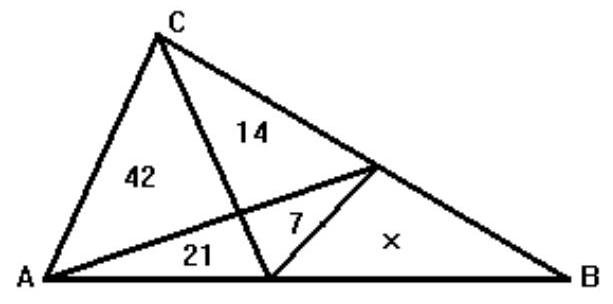
\includegraphics[max width=\textwidth, center]{2024_11_21_8382c39608adb6b5288cg-1}

\section*{ZADANIE 2.}
Oblicz \(\sqrt{37-20 \sqrt{3}}+\sqrt{13-4 \sqrt{3}}\).

\section*{ZADANIE 3.}
Rozwiąż układ równań

\[
\left\{\begin{array}{l}
5 x(x+y+z)=4 \\
2 y(x+y+z)=6 \\
4 z(x+y+z)=4
\end{array}\right.
\]

\section*{ZADANIE 4.}
W grupie 300 studentów każdy jest matematykiem, chemikiem lub fizykiem. Połowa fizyków zajmuje się chemią, połowa chemików zajmuje się matematyką, a połowa matematyków to fizycy. Wiedząc, że żaden fizyk nie zajmuje się chemią i matematyką, odpowiedz, z ilu osób składają się te grupy.

\section*{ZADANIE 5.}
Liczbę czterocyfrową pomnożono przez 9 i otrzymano liczbę czterocyfrową zapisaną za pomocą tych samych cyfr w odwrotnej kolejności. Jaka to liczba?


\end{document}